\documentclass[tikz]{standalone}
\usetikzlibrary{arrows}
\begin{document}
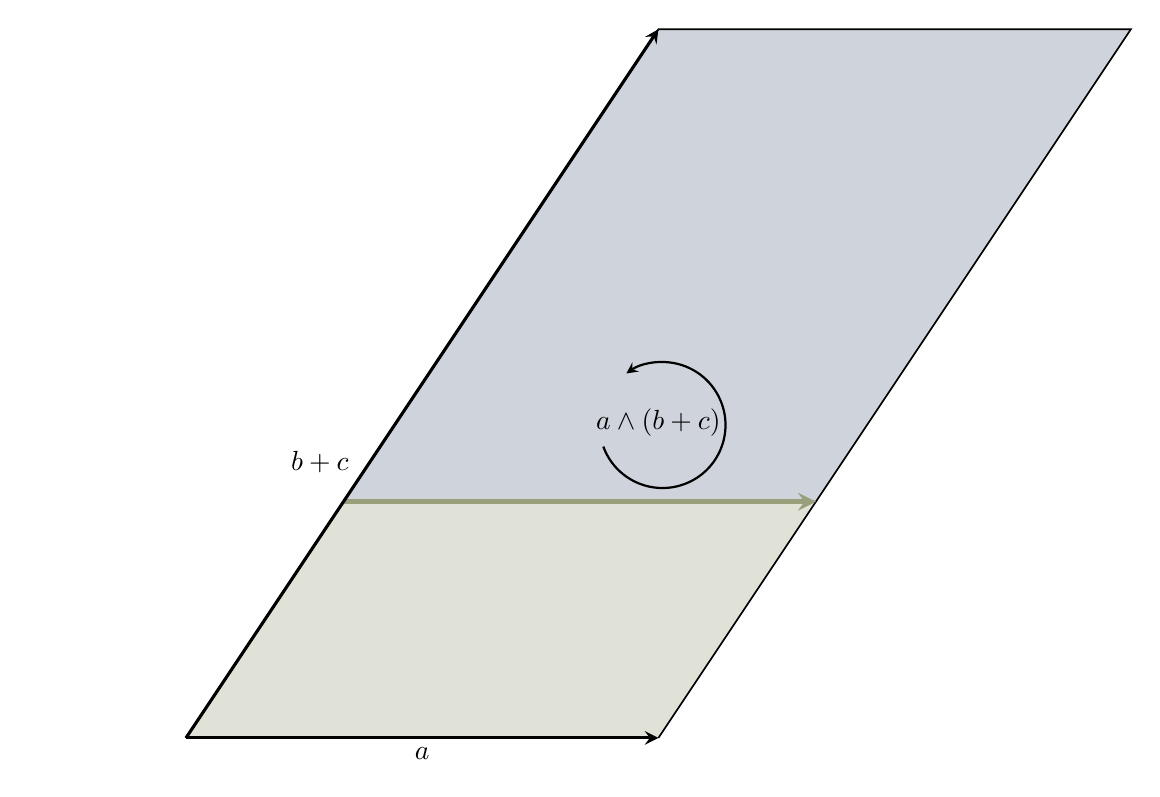
\begin{tikzpicture}[scale=1.0]
% ------------------------------------------------ lin_alg theme colors
\definecolor{la_white}{RGB}{233,235,223} %#E9EBDF
\definecolor{la_dark}{RGB}{59,54,81}     %#3B3651
\definecolor{la_gray}{RGB}{96,112,139}   %#60708B
\definecolor{la_tan}{RGB}{152,159,122}   %#989F7A

%
%  a=(6,0), b=(-8,3), bc=(2,3), c =(6,9)
%
%

\fill[line width=0.6pt,color=la_tan,fill=la_tan,fill opacity=0.3]   (2,3) -- (0,0) -- (6,0) -- (8,3) -- cycle;
\fill[line width=0.6pt,color=la_gray,fill=la_gray,fill opacity=0.3] (2,3) -- (6,9) -- (12,9) -- (8,3) -- cycle;

\draw [line width=0.6pt,color=black] (6,0)-- (8,3) -- (2,3) -- (0,0);
\draw [line width=0.6pt,color=black] (2,3) -- (6,9) -- (12,9) -- (8,3);
\draw [line width=0.6pt,color=white,opacity=0] (-2,3) -- (12,9) -- (8,3);

\draw [line width=1.8pt,color=la_tan,>=stealth,->] (2,3) -- (8,3);
% ---------------------------------------------  Vectors and Vector Labels
\draw [line width=0.4mm,>=stealth,->] (0,0) -- (6,0);
\draw [line width=0.4mm,>=stealth,->] (0,0) -- (6,9);


\draw[color=black] (3,-0.2)     node {$a$};
%\draw[color=black] (-5,1.5)     node {$b$};
%\draw[color=black] (0,6.8) node {$c$};
\draw[color=black] (1.7,3.5) node {$b+c$};

%\draw[color=black] (-2.5,2) node {$a \wedge b$}; \draw[thick,color=black,>=stealth,->] (-3,1.7) arc (-160:125:0.6);
%\draw[color=black] (0,5) node {$a \wedge c$};    \draw[thick,color=black,>=stealth,->] (-0.5,4.7) arc (-160:125:0.6);
\draw[color=black] (6,4) node {$a \wedge (b+c)$};\draw[thick,color=black,>=stealth,->] (5.3,3.7) arc (-160:125:0.8);

\end{tikzpicture}
\end{document}